\documentclass[12pt]{article}

%% Language and font encodings
\usepackage[english]{babel}
\usepackage[utf8x]{inputenc}
\usepackage[T1]{fontenc}
\usepackage{wrapfig}

%% Sets page size and margins
\usepackage[letterpaper,top=1in,bottom=1in,left=1in,right=1in,marginparwidth=1in]{geometry}

%% Useful packages
\usepackage{amsmath}
\usepackage{amssymb}
\usepackage{graphicx}
\usepackage[colorinlistoftodos]{todonotes}
\usepackage[colorlinks=true, allcolors=blue]{hyperref}

\newcommand{\Contributors}[1]{ {\footnotesize [\textit{#1}]}}

%A few journal ref commands
\newcommand{\apjl}{Astrophys. J. Lett.}
\newcommand{\apj}{Astrophys. J.}
\newcommand{\aap}{Astron. Astrophys.}
\newcommand{\nat}{Nature (London)}
\newcommand{\aj}{Astron. J.}
\newcommand{\prd}{Phys. Rev. D}
\newcommand{\aas}{Bull. Am. Astron. Soc.}
\newcommand{\mnras}{Mon. Not. R. Astron. Soc.}
\newcommand{\jcap}{Journal of Cosmology and Astroparticle Physics}
\newcommand{\vg}[1] {\textcolor{red}{#1}}

\title{\textbf{Astro2020 Science White Paper}\\
\vspace{0.5cm}
Cosmological Probes of Dark Matter: The Next Decade}
\date{}
\author{}

\begin{document}
\maketitle
\vspace{-2cm}
\begin{center}
\textbf{Thematic area:} Cosmology and Fundamental Physics.     
\end{center}
\vspace{0.5cm}

{\begin{tabular}{ll}
\textbf{Principal Author:} \\
Vera Gluscevic & \\
University of Florida \& Princeton University & \\
email: verag@princeton.edu\\
phone: 609-258-0720 & 
\end{tabular}

\vspace{0.5cm}
%\vfill
{\begin{tabular}{l}
\textbf{Co-Authors:}\\
Yacine Ali-Haimoud (\textit{NYU})\\
Kimberly Boddy (\textit{JHU})\\
Celine Boehm (\textit{})\\
Jens Chluba (\textit{JBCA Manchester})\\
Francis-Yan Cyr-Racine (\textit{Harvard})\\
Cora Dvorkin (\textit{Harvard})\\
Daniel Grin (\textit{Haverford})\\
Julien Lesgourgues (\textit{})\\
Vivian Poulin (\textit{})\\
Sarah Shandera (\textit{})\\
Tracy R. Slatyer (\textit{MIT})\\
\end{tabular}}
}
\vspace{7mm}
%{\begin{tabular}{l}
%\textbf{Endorsers:}\\
%%& \phantom{aaaaaaaaaaaaaaaaaaaaaaaaaaaaaaaaaaaaaaaaaaaaaaaaaaaaaa}
%\end{tabular}}



\begin{abstract}
Cosmological observations offer unique and robust avenues for probing fundamental nature of dark matter particles---they broadly test a range of compelling theoretical scenarios, often surpassing or complementing the reach of terrestrial and other experiments.
We discuss observational and theoretical advancements that will play a pivotal role in realizing a strong program of cosmological searches for the identity of dark matter in the coming decade, focusing on measurement of the CMB anisotropy and spectral distortions, and tracers of structure (such as Lyman-$\alpha$ forest, galaxies, and cosmological 21-cm signal).

\end{abstract}

\pagebreak
\section{Key Question: What is Dark Matter?}
 
Observations of the Universe, from our galactic neighbourhood, to the cosmological horizon, consistently testify that $\sim$85$\%$ of matter behaves as cold non-collisional fluid that sources gravitational potentials and underpins structure on virtually all observable scales.
\textbf{Over the past decades, it was confidently established that the main constituents of the dark matter (DM) component \textit{cannot} be any known baryonic particles.}
The existence of DM thus implies new physics whose investigation centrally drives research at the intersection of modern astrophysics and particle physics. 

Following its discovery, a versatile range of laboratory experiments was built worldwide to directly detect and/or produce some of the best-motivated particle candidates that could account for cosmological DM: WIMPs, WIMP-like particles, axions, etc; so far, this effort is without success.
Astrophysical and cosmological observations provide the only evidence for the existence of DM, and source a large portion of what is known about its properties---its stability on cosmological time scales, its apparent non-collisional nature, and its central role in the formation and growth of structure.
Recently, those observations have also emerged as a powerful probe of DM microphysics, complementary in reach to laboratory experiments.

%%%%%%%%%%%%%%%%%
\begin{wrapfigure}{r}{0.5\textwidth}
\begin{center}
\vspace{-0.9cm}
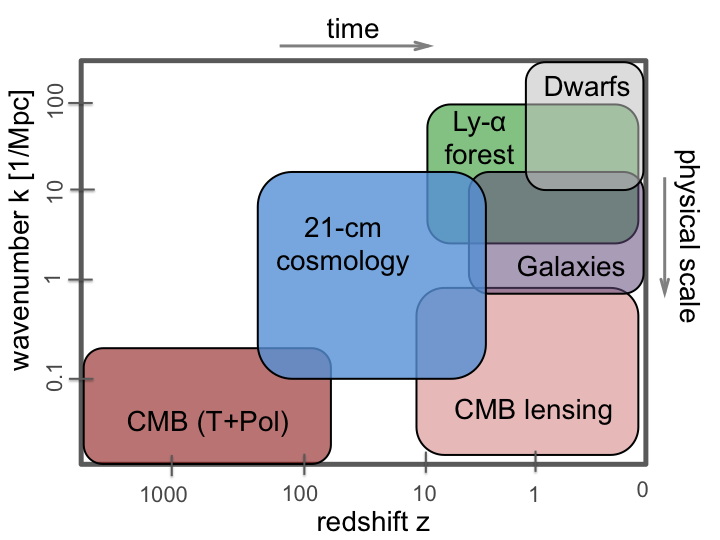
\includegraphics[width=0.5\textwidth]{scales.png}
\end{center}
\vspace{-0.8cm}
\caption{Approximate coverage of cosmological epochs and physical scales for different observables (spectral distortions are omitted for compactness of presentation; their origin is outside the LHS border of the plot).}
\vspace{-0.2cm}
\label{fig:scales}
\end{wrapfigure}
%%%%%%%%%%%%%%%%% 
We focus on cosmological searches, whose key goal is to detect the effects of DM interactions on structure and thermal history of the Universe, and use them to pin down particle identity of DM.
\textbf{Cosmology is a versatile tool that can test broad classes of theoretical scenarios}: DM interactions with known particles (baryons, photons, and neutrinos), interactions within the DM sector itself, and DM annihilations and decays.\footnote{We note that other science white papers focus on other scenarios in which DM consists of ultra-light axion-like particles, warm DM, primordial black holes, etc.}
\textbf{The next decade of observations will see a tremendous leap in sensitivity to each of them} (in some cases, by many orders of magnitude in DM mass and interaction cross sections).
Multiple observables---cosmic microwave background (CMB) anisotropy and spectral distortions, large-scale and structure tracers, and objects in our Galactic neighbourhood---can all probe the same underlying microphysics throughout cosmic history, on a broad range of physical scales (Fig.~\ref{fig:scales}).
\textbf{Establishing DM signal discovery and robustly testing its fundamental nature will rely on confirmation and consistency checks between different data sets.}
This will necessitate progress in understanding of synergies and complementarities between observables, and development of frameworks that enable their joint analyses to probe the same underlying microphysics.
In addition, DM search program with next-generation cosmological data will rely on accurate theoretical treatments of formation and evolution of small-scale structure in non-standard cosmologies, and modeling of baryonic and other non-linear effects that present potential systematic uncertainty in DM parameter inference \cite{2019arXiv190201055D,2018PhRvD..98h3540M,2019PhRvD..99b3523A}.
We review strengths, caveats, and future promise of a range of cosmological probes in search for the identity of DM, and conclude with a list of advancements that will play a pivotal role in this program in the coming decade.
%%%%%%%%%%%%%%%%%%%%%%%%%%%%%%%%%%%%%%%%%%%%%
\vspace{-0.4cm}
\section{Theory and Observations}
\label{sec:thobs}
\vspace{-0.2cm}
\subsection{Scattering with Baryons}

In the standard model of cosmology DM is non-collisional, but elastic scattering between DM and visible particles is commonplace in some of the best-motivated DM models, including the WIMPs and WIMP-like particles.
For this reason, the most sensitive terrestrial DM searches with direct detection experiments are looking for scattering of Galactic-halo DM on nuclei in underground targets.
However, the same scattering processes can occur in a cosmological setting and lead to an exchange of heat and momentum between DM and baryons, absent in the standard (non-collisional) cosmology. 
This can affect both the thermal history of the Universe and the evolution of cosmological perturbations, captured by various observables.

%%%%%%%%%%%%%%%%%%%%%
\textbf{CMB spectral distortions.} 
DM can drain heat from the primordial plasma, by scattering with either protons, electrons, or photons, in the early Universe \cite{AliHaimoud_15}.
The exchange occurring later than two months after the Big Bang cannot fully thermalize, and thus leads to distortions of the CMB frequency spectrum away from a perfect blackbody \cite{Hu_96,2012MNRAS.419.1294C}.  
%The rate of heat transfer is proportional to the \emph{number density} of DM particles, and hence inversely proportional to their mass. 
The CMB frequency spectrum is most sensitive to light particles that thermally decouple as early as $z \sim 2 \times 10^6$.
The existing COBE FIRAS measurements provide upper limits on DM-baryon and DM-photon interactions, for DM masses lower than $\sim 0.1$ MeV. 
These limits are similarly stringent, but independent of those derived from CMB anisotropy from \textit{Planck}.
Future measurements that can detect a fractional distortion of order $\sim 10^{-8}$ would be sensitive to interacting DM particles as massive as $\sim 1$ GeV. 
Spectral distortions in conjunction with power-suppression in CMB anisotropy in future data could yield robust evidence for DM physics taking place in the very early Universe.

%%%%%%%%%%%%%%%%%%%%%%%%%%%%%%%%%%%%
\textbf{CMB anisotropy.} 
Scattering in the early Universe (prior to recombination at $z\sim 1100$) leads to momentum transfer and a drag force between the DM and the baryon fluids.
This results in power suppression in density fluctuations, more prominent on progressively smaller scales (with an amplitude proportional to the strength of the scattering interaction).
As perturbations grow, the lack of small-scale structure propagates into all visible tracers of matter, and shows up in observables that span cosmic history (Fig.~\ref{fig:scales}).
%%%

\textit{Planck} measurements of the CMB temperature anisotropy currently provide the most pristine cosmological bound on the DM-baryon scattering cross section~\cite{Boddy:2018kfv,Gluscevic:2017ywp,Boddy:2018wzy,Xu:2018efh,Slatyer:2018aqg,Dvorkin:2013cea}; they already sensitively probe DM interactions as far back in time as when the Universe was a thousand years old.
However, the first high-signal-to-noise measurements of the CMB polarization and lensing on small ($\lesssim$arcminute) angular scales---to be delivered by the next-generation CMB experiments---can enable a leap in sensitivity to DM scattering by up to \textit{several orders of magnitude}~\cite{Li:2018zdm,2018arXiv180807445T,Abazajian:2016yjj,2019arXiv190210541H}.
Interestingly, the effects of DM-baryon interactions are distinct from other new physics targeted by future CMB experiments (such as, for example, the neutrino mass and ultra-light particles).
Furthermore, DM-baryon scattering is insensitive to uncertainties on cosmological parameters, and can be robustly probed with the CMB.
However, in spite of its robustness, the CMB has a limited grasp of small scales where the effects of interactions are more prominent; small scales are accessible to other observables, but are more prone to modeling and measurement systematic uncertainty.

\textbf{Lyman-$\alpha$ forest.} 
For example, the Lyman-$\alpha$ forest measurements from SDSS trace the matter power spectrum on scales of about 1 Mpc comoving; their analysis provided the most stringent to-date cosmological bound on DM-baryon interactions, surpassing the reach of the CMB  \cite{Xu:2018efh,Dvorkin:2013cga}.
This bound implies that a baryon within a galaxy like the Milky Way does \textit{not} scatter with DM over the age of the galaxy.
There is vast room for improvement with future spectroscopic surveys that could reconstruct even smaller scales with similar measurements.
However, inference of fundamental physics from these measurements will crucially rely on accurate modeling of the Lyman-$\alpha$ forest and non-linear evolution of small scales.
Consistency checks and joint analyses with high-precision CMB measurements and other probes may help alleviate such uncertainties in future data.

%%%%%%%%%%%%%%%%%%%%%%%%%%
\textbf{21-cm cosmology.} 
Over the coming decade, measurements of the hyperfine 21-cm line transition in atomic hydrogen gas during cosmic Dark Ages and cosmic reionization ($10<z<1000$) will start to probe redshifts far beyond the reach of current observations.
The strength of the 21-cm signal is proportional to the difference between the temperature of the hydrogen gas (baryons) and that of the CMB, and acts as a calorimeter that can probe thermal history at redshifts as high as $\sim 200$.
If DM-baryon scattering occurs \textit{after} recombination is complete, it can alter thermal evolution of baryons in the epoch originating the 21-cm signal. 
The sky-averaged signal and its fluctuations are both sensitive to this effect \cite{Munoz_15, Barkana_18, Fialkov_18, Munoz_18}.
Such a late-time scattering scenario, for example, arises if DM particles carry a small electric charge and exhibit Coulomb-like interactions (``millicharged'' DM).
This scenario is simple and well-motivated, but challenging to probe in direct detection experiments and is an excellent example of a model where cosmological probes may present an optimal detection channel.
However, the cosmological 21-cm signal is exceptionally hard to detect due to the size of galactic foreground emission at the same frequencies. 
As was recently demonstrated on the example of the recent results from EDGES, a combination of probes is essential for interpretation of anomalies in terms of new physics \cite{Barkana:2018lgd,Kovetz:2018zan,Berlin:2018sjs}. 

%%%%%%%%%%%%%%%%
\textbf{Galaxies.}
Galaxies (and their satellites) trace matter power spectrum on even smaller scales (and in the local Universe), and thus hold a bold promise as a future probe of DM physics \cite{2019arXiv190201055D}.
Given the physical scales involved, studies of dwarfs, in particular, could unlock orders of magnitude improvement in sensitivity to DM interactions, compared to high-redshift and large-scale probes discussed earlier.
However, robust inference of fundamental physics from studies of galaxies will crucially depend on improvements in modeling and numerical simulation of their formation, non-linear growth, and baryonic effects in cosmologies with non-standard DM---a challenge that will need much attention in the coming decade.\footnote{Observables such as galaxy clustering and weak lensing are a large subject and a prime focus of other science white papers.}

%%%%%%%%%%%%%%%%%%%%%%%%%%%%%%%%%%%%%%%%%%%%%%%
%\vspace{-0.3cm}
\subsection{Scattering with Neutrinos}

Neutrinos reside in the least well understood part of the Standard Model of particle physics; indeed, non-vanishing neutrino masses require new physics to explain. 
Recently, terrestrial neutrino experiments and probes of astrophysical neutrinos have seen a number of intriguing anomalies that may indicate new physics \cite{2018arXiv180512028M, 2018arXiv180909615F}.
The idea that DM may communicate with visible matter through interactions with neutrinos is an intriguing possibility. 
However, laboratory tests of this scenario are currently impossible.
On the other hand, neutrinos are cosmologically important, owing to their high abundance (hundreds per cm$^3$ today).

If neutrinos efficiently scatter with DM in the very early Universe, after the standard neutrino decoupling takes place ($\sim 1$ sec after the Big Bang), DM-neutrino fluid undergoes acoustic oscillations and diffusion damping, and is smoother than ordinary free-streaming neutrinos (and has a smaller sound speed).
This is captured in the CMB anisotropy as a suppression of power and a shift of the acoustic peaks towards smaller angular scales, and is used to sensitively probe DM-neutrino scattering with \textit{Planck} data \cite{Boehm:2001hm,Mangano:2006mp,Escudero:2015yka,DiValentino:2017oaw,Diacoumis:2018ezi}.
The suppression of small-scale power in matter fluctuations that also arises in this scenario is best probed by visible tracers of even smaller scales.
The best current bounds on DM-neutrino scattering come from Lyman-$\alpha$ forest observations \cite{Wilkinson:2014ksa}.
Just like in the case of DM-baryon scattering, future CMB, Lyman-$\alpha$, and galaxy surveys will substantially increase sensitivity to DM-neutrino scattering by probing perturbations and structure on even smaller scales.

%%%%%%%%%%%%%%%%%%%%%%%%%%%%%%%%%%%%%%%%%%
\vspace{-0.3cm}
\subsection{Annihilation and Decay}

If DM interacts with visible particles, it may also annihilate or decay and that way further alter the thermal history of the Universe. 
If annihilation or decay products include electromagnetically interacting particles, these particles and their decay products can generically heat and/or ionize the baryonic gas.
Cosmological searches have distinct advantages over classic indirect searches for DM annihilation and decay, as they do not suffer from astrophysical backgrounds and large uncertainties in the distribution of DM in the target systems.
Furthermore, they can probe processes which have no detectable signals in terrestrial-scale experiments and in the local Universe--for example, the decay of metastable species with lifetimes comparable to the age of the Universe, and decay of DM particles into invisible channels, such as neutrinos or new dark particles \cite{Poulin:2016nat,Poulin:2016anj}. 

Increasing the ionization fraction near the time of recombination can affect the CMB anisotropy \cite{Adams:1998nr,Chen:2003gz, Padmanabhan:2005es}. 
\textit{Planck} measurements of CMB temperature and polarization anisotropy on degree angular scales provided some of the strongest and most robust bounds on annihilations and decays of sub-GeV DM, complementing indirect searches that probe heavier DM candidates \cite{Aghanim:2018eyx,Slatyer:2016qyl}. 
Measurements from the next-generation ground-based CMB experiments can improve sensitivity to DM annihilation cross section and lifetime by a factor of several.
%In addition, heat transfer and production of secondary low-energy photons could also distort the CMB blackbody spectrum by a small fraction ($\sim 10^{-9}-10^{-10}$) \cite{Chluba:2013wsa,Chluba:2016bvg}.
Furthermore, as discussed in context of DM-baryon interactions, future observations of the cosmological 21-cm signal from atomic hydrogen can sensitively track gas temperature during cosmic Dark Ages and around the epoch or Reionization.
As such, they can capture any new energy injection from DM decays and annihilations in the post-recombination Universe, likely surpassing the sensitivity of the CMB anisotropy to the same processes \cite{Furlanetto:2006wp,Valdes:2007cu,Evoli:2014pva,Lopez-Honorez:2016sur,Poulin:2016anj}. 

%%%%%%%%%%%%%%%%%%%%%%%%%%%%%%%%%%%%%%%%%%%%%%%%
\vspace{-0.4cm}
\subsection{Interactions with Dark Radiation}

Models in which the dark sector is complex and contains not only dark matter, but also dark radiation (DR) that interacts with DM particles, are motivated in several ways: they generically arise in theories proposed to explain the hierarchy problem of the Standard Model of particles \cite{Arkani-Hamed:2016rle, Chacko:2018vss}; they could explain the anomalously low large-scale amplitude of matter fluctuations seen in some weak-lensing surveys \cite{Lesgourgues:2015wza,Chacko:2016kgg,Buen-Abad:2017gxg,Krall:2017xcw}; they present a specific case of self-interacting DM, an attractive potential solution for putative anomalies on sub-galactic scales, such as the missing-satellite problem \cite{Tulin:2012wi,Tulin:2013teo,Kaplinghat:2015aga,Bullock:2017xww}. 
Cosmology offers a unique way to probe yet-unknown DM-DR interactions, especially if DM resides in a secluded dark sector (featuring only weak coupling to known particles).

Similar to how photon pressure prohibits growth of baryon fluctuations until recombination, DM interacting with DR in the early Universe experiences suppressed growth of structure, as compared to a scenario with no DR. 
The resulting suppression of power is captured in the CMB anisotropy and all tracers of large-scale structure (similar to the case of DM-baryon interactions): galaxy clustering, galaxy weak lensing, Lyman-$\alpha$ forest, and cosmological 21-cm signal \cite{Boehm:2001hm,Cyr-Racine:2013fsa,Cyr-Racine:2015ihg}. 
Notably, cosmological signatures of DR are distinct from signatures of relativistic particles that do not couple to DM, such as the standard free-streaming neutrinos~\cite{Bashinsky:2003tk,Follin:2015hya,Baumann:2015rya}.
High-precision measurements of small-angular-scale CMB polarization anisotropy with the next-generation ground-based experiments could robustly detect or rule out DM-DR interactions taking place in the early Universe, even in the case where only a small fraction (less than $5\%$) of the overall DM density couples to DR. 
As in the previously discussed theoretical scenarios, galaxies, Lyman-$\alpha$ forest, and 21-cm observations could probe even smaller scales and earlier times. 

\vspace{-0.4cm}
\section{Recommendations}
\label{sec:recommendations}
\vspace{-0.2cm}
Next decade of cosmological observations will open unique and robust avenues to broadly probe fundamental nature of dark matter particles in context of many compelling theoretical scenarios, complementing the reach of terrestrial experiments.
The following advancements will play a pivotal role in realizing a strong program of cosmological searches for the identity of dark matter in the coming decade:
\vspace{-0.cm}
\begin{itemize}
    \item \textbf{Observations:}
    \begin{itemize}
        \item Next-generation measurements of small-angular-scale CMB anisotropy.
        \item Measurements of thermal history (global 21-cm signal, CMB spectral distortions).
        \item Surveys of matter-power-spectrum tracers (21-cm tomography, Lyman-$\alpha$ forest, galaxy clustering and weak lensing).
        \item Near-field cosmology (local probes of small-scale structure).
    \end{itemize}
    \vspace{-0.2cm}
    \item \textbf{Theory and analysis:}
    \begin{itemize}
        \item High-accuracy theoretical treatment of cosmological DM signals on small scales.
        \item Simulation and modeling of non-linear growth in novel DM cosmologies.
        \item Understanding of baryonic systematic effects in DM-related inference.
        \item Frameworks for joint analyses of cosmological probes.
        \end{itemize}
\end{itemize}
\bibliographystyle{ieeetr}
\bibliography{DMCosmology}

\end{document}